\chapter{Super-Kamiokande Gadolinium Upgrade}\label{chp:superkgdupgrade}


\section{Physics motivation behind Super-Kamiokande Gadolinium Upgrade}

In order to be able to possibly observe the supernova relic neutrino (SRN) flux, also known as diffuse supernova neutrino background (DSNB) flux it was proposed that Gadolinium (Gd) should be added to the the water in Super-Kamiokande. Natural isotopes of gadolinium have large thermal neutron capture cross sections. As a result of this, when neutrons are captured on them there is a cascade of gamma rays that occurs, with an energy totalling ~8 MeV, whereas neutron capture that occurs on hydrogen produces a single 2.2 MeV gamma ray. Two such natural isotopes, Gd-155 and Gd-157 have thermal neutron capture cross sections of 60740 barns and 253700 barns respectively, while the thermal neutron capture cross section of hydrogen is just 0.329 barns \cite{meoMeasurementNeutronCapture}. The Super-Kamiokande with Gadolinium experiment, formerly known as GADZOOKS! (Gadolinium Antineutrino Detector Zealously Outperforming Old Kamiokande, Super!) was proposed in 2003, which stated the intention of enriching Water Cherenkov detectors with water soluble gadolinium salt. The ultimate aim is to load a total amount of gadolinium in the form of gadolinium sulphate octahydrate($$
\mathrm{Gd}_{2}\left(\mathrm{SO}_{4}\right)_{3} \cdot 8 \mathrm{H}_{2} \mathrm{O}$$) in Super-Kamiokande which equates to 0.2\% of Gd by mass, which would allow for 90\% neutron capture efficiency. The ability to tag neutrons efficiently in Super-Kamiokande will benefit multiple physics topics, not only for the aforementioned observation of SRN flux, but also for analyses involving atmospheric neutrinos and proton decay. 
\newline

A massive amount of energy is relased when a core-collapse supernova (SN) occurs, about $10^{46}$ J. The vast majority of this energy (99\%) is released in the form of neutrinos, and due to neutrinos interacting with matter only very weakly, these traverse space with barely any attenuation. The interaction through which neutrino detectors such as Super-Kamiokande detect SRN flux is through inverse beta decay (IBD), shown in Equation \ref{eq:IBD_equation}. 

\begin{equation}
    \bar{\nu}_{e}+p \rightarrow n+e^{+}
\label{eq:IBD_equation}
\end{equation}

Due to the large cross section of the interaction, these events constitute about 88\% of the total number of events in the detector \cite{martiEvaluationGadoliniumAction2020}. With efficient neutron tagging in Super-Kamiokande, the backgrounds (charged current interactions and muon spallation) in the search for SRN flux neutrinos would be largely reduced. The neutral current quasielastic (NCQE) background would still remain due to the way the gamma rays arising from neutron capture mimic the signal of the inverse beta decay (IBD) reactions: a schematic of both NCQE and IBD reactions are shown in Figure \ref{fig:NCQE_IBD}. The measurement of the NCQE interactions using T2K beam flux can aid in understanding this background more due to the T2K flux peak being near the atmospheric neutrino flux peak (~600 MeV). 


\begin{figure}[H]
    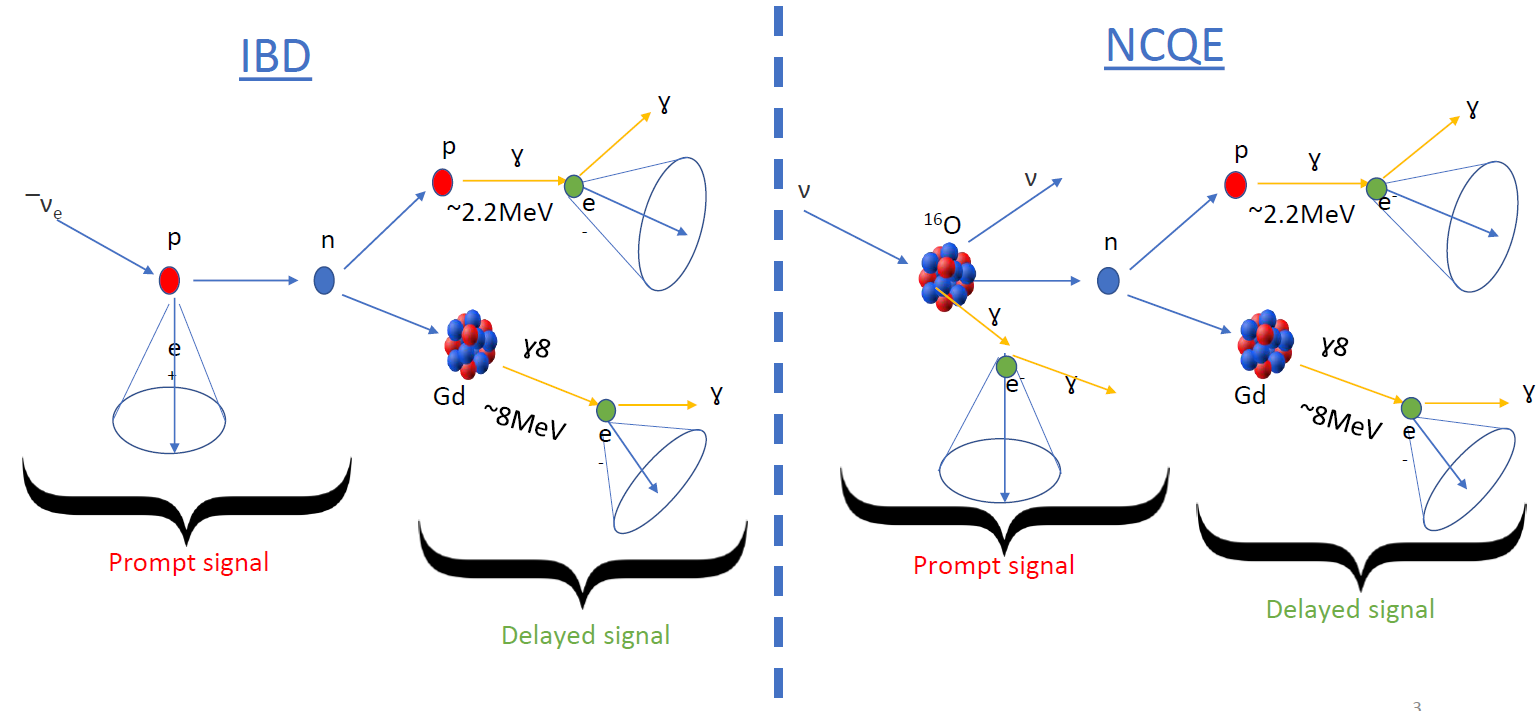
\includegraphics[width=\textwidth]{Figures/schematic.png}
\caption{Schematic showing the IBD and NCQE interaction mechanisms}
\label{fig:NCQE_IBD}
\end{figure}


Efficient neutron tagging aids information about neutrino energy and neutrino interaction type, and when it comes to studying atmospheric neutrino oscillations, accurate neutrino energy reconstruction is particularly important. Figure \ref{fig:atm_nu_energy} shows the fraction of non-visible energy as a function of the number of tagged neutrons from simulations of atmospheric neutrino interactions at Super-Kamiokande. Here $E_{\nu}$ is the energy of the atmospheric neutrino and $E_{vis}$ is the energy that is reconstructed from charged particles. Due to these neutrinos interacting with nuclei in the detector, more neutrons are produced, and with efficient neutron tagging on gadolinium the neutrino energy can be properly reconstructed. 

\begin{figure}[H]
    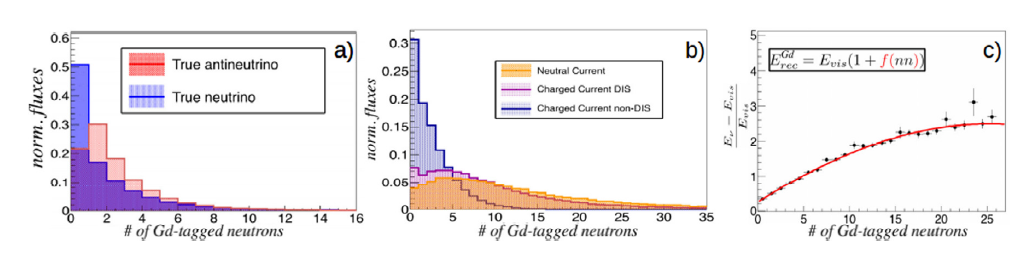
\includegraphics[width=\textwidth]{Figures/atm_recon_energy.png}
\caption{MC study of (a) neutron multiplicity production for $\nu$ and ${\bar{\nu}}$, (b) neutral current, charged current and deep and non-deep inelastic scattering, (c) the correction to the visible energy as a function of neutrino multiplicity. Taken from \cite{martiEvaluationGadoliniumAction2020}.}
\label{fig:atm_nu_energy}
\end{figure}


Proton decay searches benefit from the addition of gadolinium to Super-Kamiokande because the main background to proton decay analyses come from atmospheric neutrino interactions, due to Figure \ref{fig:atm_nu_energy} showing that atmospheric neutrinos cause at least one neutron to be produced. 

\section{The EGADS project}

In 2009, prior to the additon of gadolinium in Super-Kamiokande, the EGADS (Evaluating Gadolinium's Action on Detector Systems) project was used to evaluate how the inclusion of gadolinium sulphate octahydrate would affect water quality and detector components inside Super-Kamiokande and their analyses. It was also used to observe how to reduce the visible neutron background from spallation and neutrons from fission chains from the uranium and thorium impurities in the gadolonium sulphate. EGADS is a cylindrical 200 ton stainless steel tank in a cavern near Super-Kamiokande and has its own water purification system and gadolinium sulphate octahydrate dissolving system. 

Observing the impact the addition of gadolinium sulphate octahydrate had on the water quality and components was especially crucial, and after loading 0.2\% gadolinium sulphate into the the EGADS tank in 2013, 240 PMTs were installed into the detector. 224 of these are the 50 cm Super-Kamiokande inner detector PMTs, with 60 of these having the same FRP and acrylic covers as the inner detector PMTs. Much like Super-Kamiokande, the active photocoverage for EGADS is ~40\%, with the inside walls of the detector also being covered in black polyethylene terephthalate sheets. However, unlike Super-Kamiokande, there is no outer detector in EGADS. Figure \ref{fig:EGADS_PMT} shows the PMT map for the EGADS detector along with the PMT types. Along with the PMTs which are identical to the ones inside Super-Kamiokande, EGADS also contains PMTs which are used for research and developement for use inside Hyper-Kamiokande \cite{martiEvaluationGadoliniumAction2020a}.

\begin{figure}[H]
    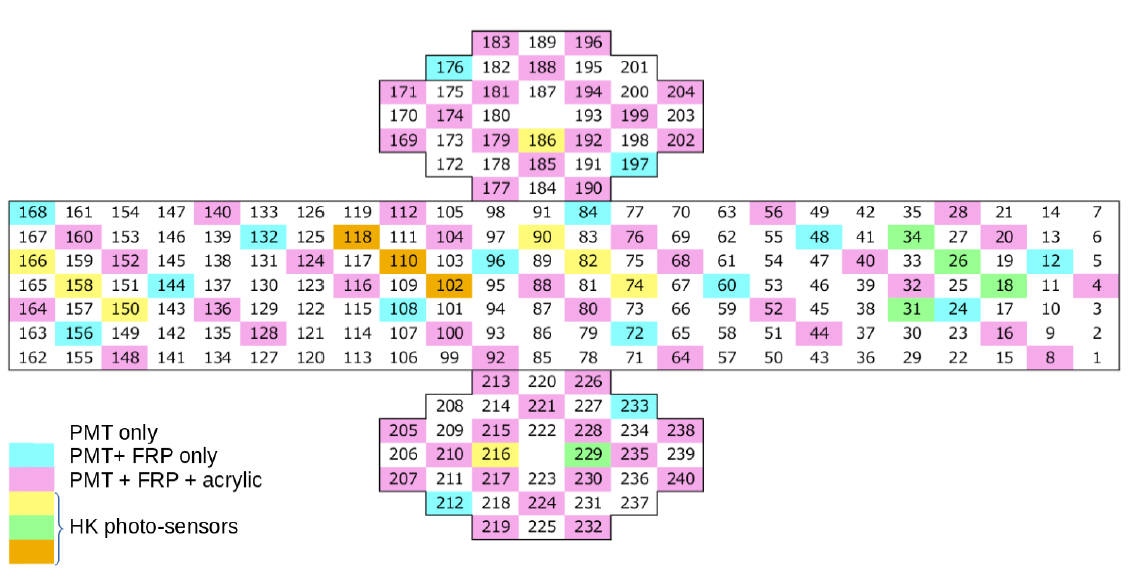
\includegraphics[width=\textwidth]{Figures/egads_pmt_map.png}
\caption{Map of unrolled cylindrical EGADS detector with PMT types. Taken from \cite{martiEvaluationGadoliniumAction2020a}.}
\label{fig:EGADS_PMT}
\end{figure}

Measurements regarding neutron tagging were also taken using an Americium/Beryllium (Am/Be) source placed inside EGADS. Using an Am/Be neutron source to observe gadolinium's efficacy with respect to tagging neutrons is feasible because the Am/Be source decays as in Equation \ref{eq:ambe_decay}. It produces a prompt 4.4 MeV gamma ray alongside a neutron during it's decay process, and as a result the prompt 4.4 MeV signal can serve as a trigger signal, while the following hundreds of microseconds can be used as a timing window within which to scan for the neutron. Due to its similarity to the neutral current quasieleastic events studied in the analysis in this thesis, it can serve as a helpful control sample and is used in the calculation of the detector response uncertainty in Chapter 7.

\begin{equation}
\begin{array}{c}
\alpha^{9} \mathrm{Be} \longrightarrow^{12} \mathrm{C}^{*} \mathrm{n} \\
{ }^{12} \mathrm{C}^{*} \longrightarrow{ }^{12} \mathrm{C} \gamma(4.4 \mathrm{MeV})
\end{array}
\label{eq:ambe_decay}
\end{equation}

The delayed neutron capture time from an Am/Be source used in EGADS with the gadolinium sulphate concentration of 0.2\% is shown in Figure \ref{fig:EGADS_ambe_capture}. Here, we can see that the neutron capture time from the data is 29$\pm$0.3 $\mu$s and for the Monte Carlo it is 30$\pm$0.8 $\mu$s.

\begin{figure}[H]
    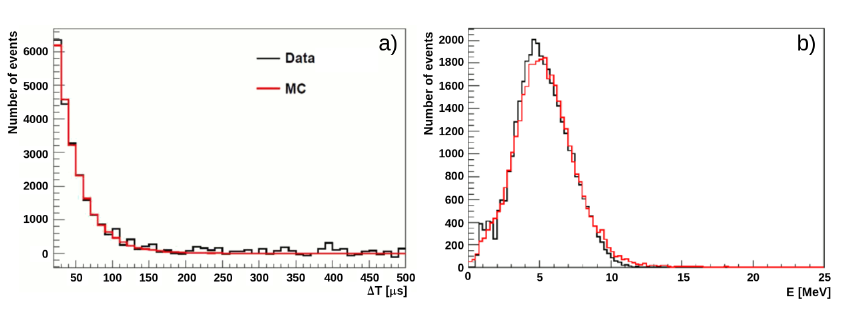
\includegraphics[width=\textwidth]{Figures/egads_ambe.png}
\caption{a) Delayed neutron capture time from prompt event with Am/Be source. (b) Reconstructed energy from gamma rays after neutron capture.}
\label{fig:EGADS_ambe_capture}
\end{figure}

EGADS water transparency and and gadolinium sulphate concentration was monitored daily to ensure similarity to ensure no negative effects to the detector components. Figure \ref{fig:egads_transparency} shows the transparency and concentration from bottom, top and centre sampling ports in EGADS, with the blue band being typical water transparency values for Super-Kamiokande. It shows that the water transparency values remain comparable to Super-Kamiokande values and that there is very little variation from the final target gadolinium sulphate concentration, as there is little variation from the black dashed line. 

\begin{figure}[H]
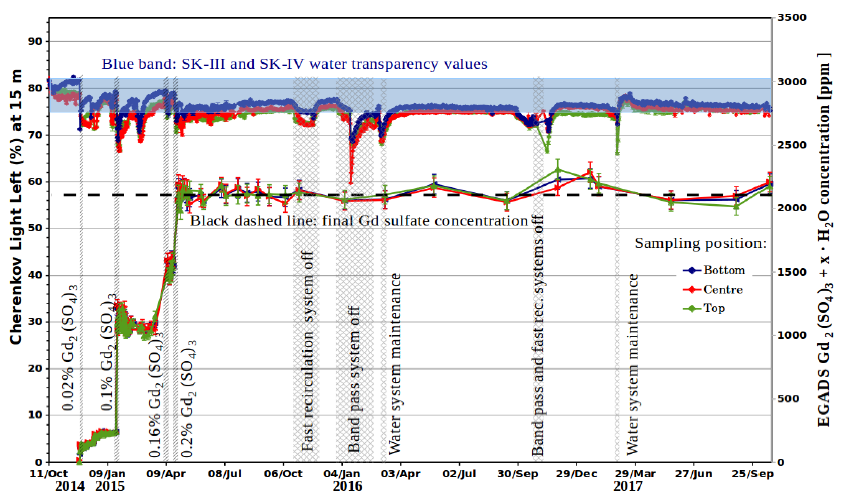
\includegraphics[width=\textwidth]{Figures/egads_concentration.png}
\caption{The upper lines are Cherenkov light left (\%) and the lower three lines represent gadolinium sulphate concentration. The blue, red and green lines represent measurements taken from the bottom, centre and top sampling ports, respectively. Taken from \cite{martiEvaluationGadoliniumAction2020a}}
\label{fig:egads_transparency}
\end{figure}

EGADS also represented the most realistic possible soak test, and after two and a half years of running EGADS was emptied in November 2017 to check the condition of the inner structure and the photomultiplier tubes. There was no deteriation of any of the components, which was an excellent sign for a detector designed to so closely resemble the conditions for the Super-Kamiokande Gadolinium upgrade. 

\section{Gadolinium loading into Super-Kamiokande}

After the success of EGADS, the Super-Kamiokande Gadolinium project was formed in 2015 when the final goal of adding 0.2\% gadolinium sulphate octahydrate by mass to the detector. 10\% of the target concentration was then loaded into Super-Kamiokande from July 14th to August 17th 2020. The details of the various aspects of the gadolinium loading are mentioned in the next subsections: the SK-Gd water system, the flow of the water in the detector, and the loading of the gadolinium sulphate octahydrate powder.

\subsubsection{The SK-Gd water system}

The SK-Gd water system was designed to dissolve gadolinium sulphate octahydrate into the detector water, pass it through a ''pretreatement" system to remove contaminants from the water, and then to continously circulate it. Figure \ref{fig:skgd_water_system} shows a schematic of the system. The $$
\mathrm{Gd}_{2}\left(\mathrm{SO}_{4}\right)_{3} \cdot 8 \mathrm{H}_{2} \mathrm{O}
$$ powder is transported to a weighing hopper whch dissolves it into water held in a dissolving tank, which allows for exact amounts of the powder to be dissolved to attain the specific concentration required. The water in Super-Kamiokande is fed into a solvent tank, and then to the dissolving tank, from which it recieves the gadolinium sulphate octahydrate from the shear blender. Water from this dissolving tank mixes the powder, and this combination is sent to the pretreatment system. The design for this treatment system was successfully tested in EGADS and involves treating this solution with ultraviolet light. Positively charged impurites dissolved in the solution (such as radium ions) and negatively charged impurities (such as uranium) are removed using a cation and anion exchange resins respectively. The gadolinium loaded water is next transferred to a UV steriliser to remove bacteria introduced during the dissolving process. This pretreatement process only occurs during gadolinum octahydrate sulphate dissolution, and not during the recirculation process. The recirculation process is similar to the pretreatement process, but with ultrafiltration modules installed in the final stage, and heat exchmage units used before the water is returned to the detector, to help maintain exact control over the water temperature.

\begin{figure}[H]
    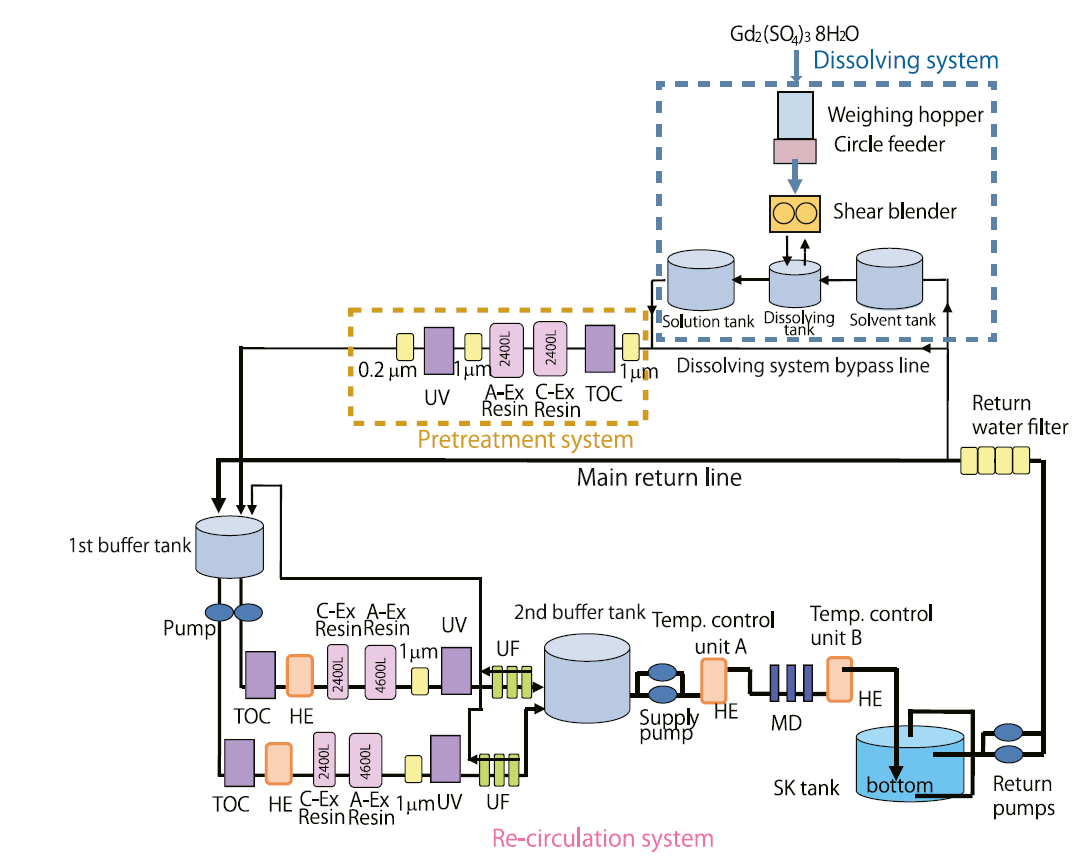
\includegraphics[width=\textwidth]{Figures/skgd_water_system.png}
    \caption{Schematic of the SK-Gd water system}
    \label{fig:skgd_water_system}
    \end{figure}

\subsubsection{Control of water parameters in SK-Gd}

Before gadolinium loading occurred, the water temperature in the tank was set at 13.9 \degree C exactly and was circulated at this temperature for about 45 days. The temperature of the ''supply water" (water sent from the water system to the detector tank) was set to a lower temperature (13.55 \degree C) as Gd-loading began. This gradient in the density between the tank water and supply water meant that spatial configuration of the Gd-loaded water could be observed, by taking the temperature of the water at different locations in the tank. Figure \ref{fig:gd_pipes} shows a schematic of the water piping during Gd dissolving for both the inner and outer detectors. 


\begin{figure}[H]
    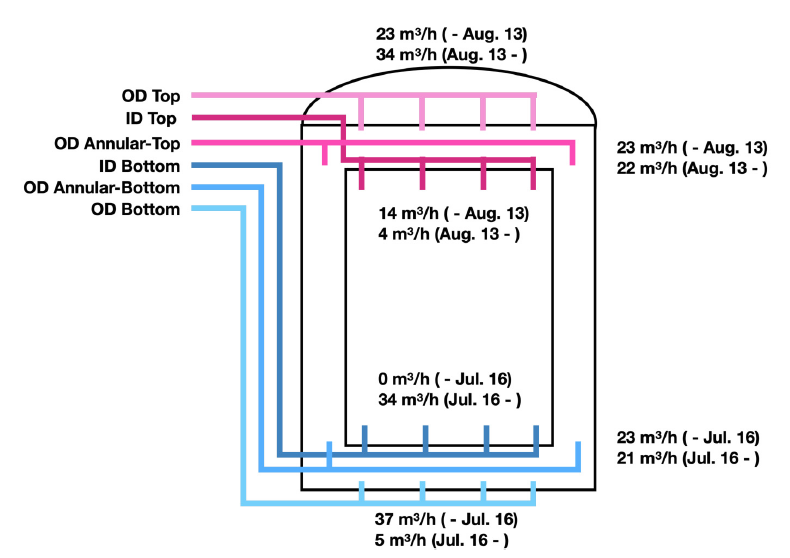
\includegraphics[width=\textwidth]{Figures/gd_pipes.png}
    \caption{Schematic of the SK-Gd water piping for both the ID and OD}
    \label{fig:gd_pipes}
\end{figure}


\subsubsection{Gd-powder specification and loading}

The acceptable background rate after the final value for Gd loading (set to be a concentration of 0.1\% Gadolinium) was set to be less than double that of the background rate for when Super-Kamioknde ran with pure water. As a result, rigorous standards of cleanliness were set for the $$\mathrm{Gd}_{2}\left(\mathrm{SO}_{4}\right)_{3} \cdot 8 \mathrm{H}_{2} \mathrm{O}$$ powder, which meant setting maximum allowed levels of radioactive impurites which are shown in Table \ref{gdpowderradiation}.


\begin{table}[H]

$\begin{array}{llll}
\hline \text { Chain } & \text { Isotope } & \text { Criterion [mBq/kg] } & \text { Physics target } \\
\hline{ }^{238} \mathrm{U} & { }^{238} \mathrm{U} & <5 & \text { SRN } \\
& { }^{226} \mathrm{Ra} & <0.5 & \text { Solar } \\
\hline{ }^{232} \mathrm{Th} & { }^{232} \mathrm{Th} & <0.05 & \text { Solar } \\
& { }^{228} \mathrm{Ra} & <0.05 & \text { Solar } \\
\hline{ }^{235} \mathrm{U} & { }^{235} \mathrm{U} & <30 & \text { Solar } \\
& { }^{227} \mathrm{Ac} /{ }^{227} \mathrm{Th} & <30 & \text { Solar } \\
\hline
\end{array}
$
\label{gdpowderradiaton}
\end{table}


\begin{figure}[H]
    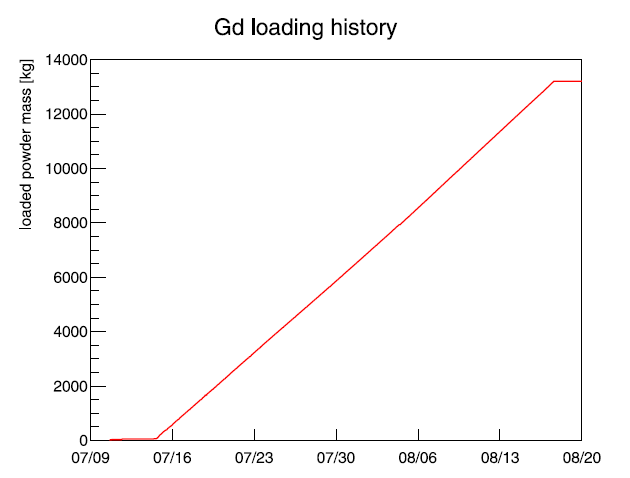
\includegraphics[width=\textwidth]{Figures/gdloadinghistory.png}
    \caption{Schematic of the SK-Gd water piping for both the ID and OD}
    \label{fig:gdloadinghistory}
\end{figure}

To sustain this very small level of impurity, the gadolinium powder batches went under routine screening at three collaboration laboratories at Boulby (UK), Canfranc (Spain), and the Kamioka Observatory. 

Figure \ref{gdloadinghistory} shows the loaded mass of gadolinium powder in Super-Kamiokande at each dissolving cycle. The loaded mass of gadolinium sulphade octahydrate powder increased linearly until the target value of 5426 kg of it dissolved in 44,878,429 kg of water in Super-Kamiokande, resulting in a gadolinium concentration of 0.011\% and a gadolinium sulphate ($\mathrm{Gd}_{2}\left(\mathrm{SO}_{4}\right)_{3}$) concentration of 0.021\%. After the loading of gadolinium sulphate powder into Super-Kamiokande, water transparency and attenuation length were continously monitored. This had also been conducted in EGADS (see previous section), but due to the flow rate of the water and method by which gadolinium is loaded into the detector being different in Super-Kamiokande, it is important to monitor these attributes in the SK-Gd upgrade as well. Figure \ref{gdattenuationlength} shows how the attenuation length of the Cherenkov light in SK-Gd varies with time: this attenuation length is measured using cosmic ray through going muons (as explained in Chapter 3). There is a clear increase in the 





